\documentclass[a4paper,12pt]{article} 
\usepackage[utf8]{inputenc} % Acentos válidos sin problemas
\usepackage[spanish]{babel} % Idioma
%\usepackage[style=biber]{biblatex}
%\addbibresource{bibliografia.bib}
%\usepackage[
%  backend=biber
%]{biblatex}
\usepackage[backend=biber, style=ieee]{biblatex}
\addbibresource{bibliografia.bib}
\usepackage{csquotes}
%\usepackage{background}
%\setlegtth{\parindent}{2px}
%\phantom{abc}
%-----------------------------------INICIO DE PACKETES------------------/
%----------------------------------------------------------------------/|
\usepackage{amsmath}   % Matemáticas: Comandos extras(cajas ecuaciones) |
\usepackage{amssymb}   % Matemáticas: Símbolos matemáticos              |
\usepackage{datetime}  % Agregar fechas                                 |
\usepackage{graphicx}  % Insertar Imágenes                              |
\usepackage{biblatex} % Bibliografía                                   |
\usepackage{multicol}  % Creación de tablas                             |
\usepackage{longtable} % Tablas más largas                              |
\usepackage{xcolor}    % Permite cambiar colores del texto              |
\usepackage{tcolorbox} % Cajas de color                                 |
\usepackage{setspace}  % Usar espacios                                  |
\usepackage{fancyhdr}  % Para agregar encabezado y pie de página        |
\usepackage{lastpage}  %                                                 |
\usepackage{float}     % Flotantes                                      |
\usepackage{soul}      % "Efectos" en palabras                          |
\usepackage{hyperref}  % Para usar hipervínculos                        |
\usepackage{caption}   % Utilizar las referencias                       |
\usepackage{subcaption} % Poder usar subfiguras                         |
\usepackage{multirow}  % Nos permite modificar tablas                   |
\usepackage{array}     % Permite utilizar los valores para multicolumn  |
\usepackage{booktabs}  % Permite modificar tablas                       |
\usepackage{diagbox}   % Diagonales para las tablas                     |
\usepackage{colortbl}  % Color para tablas                              |
\usepackage{listings}  % Escribir código                                |
\usepackage{mathtools} % SIMBOLO :=                                     |
\usepackage{enumitem}  % Modificar items de Listas                      |
\usepackage{tikz}      %                                                |
\usepackage{lipsum}    % for auto generating text                       |
\usepackage{afterpage} % for "\afterpage"s                              |
\usepackage{pagecolor} % With option pagecolor={somecolor or none}|     |
\usepackage{xpatch}    % Color de lineas C & F
%\usepackage{glossaries} %                                             
\usepackage{lastpage}       





%----------------------------------------------------------------------\|
%-----------------------------------FIN--- DE PACKETES------------------\
%\usepackage{listings}
%\lstset{
%  language=Scheme
%}

%--------------------------------/
%-------------------------------/
\usepackage[                 %   |
  headheight=15pt,  %            |
  letterpaper,  % Tipo de pag.   |
  left =1.5cm,  %  < 1 >         |
  right =1.5cm, %  < 1 >         | MARGENES DE LA PAGINA
  top =2cm,     %  < 1.5 >       |
  bottom =1.5cm %  < 1.5 >       |
]{geometry}     %                |
%-------------------------------\
%--------------------------------\

%----------------------------------------------------------------------/
%-------------------Encabezado y Pie de Pagina-----------------------/ |
%--------------------------------------------------------------------\ |
%\fancyhf{}           %                                                |

     %                                                |
%\pagestyle{fancy}

\fancypagestyle{firstpage}{  
  \fancyfoot[L]{\textsc{\textcolor{white}{\small {Fundamentos de Bases de Datos}}}}
  \fancyfoot[C]{}
  \fancyfoot[R]{\textcolor{white}{\thepage\ de \pageref*{LastPage}}} 
  \renewcommand{\footrulewidth}{1.5pt} %     | 
\xpretocmd\footrule{\color{white}}{}{\PatchFailed}
}

\fancypagestyle{fancy}{  

\fancyhead[L]{{\textcolor{white}{2024-1}}} %                         
\fancyhead[R]{\textcolor{white}{}}     % |
\fancyfoot[L]{\textsc{\textcolor{white}{\small {Fundamentos de Bases de Datos}}}}
  \fancyfoot[C]{}
  \fancyfoot[R]{\textcolor{white}{\thepage\ de \pageref*{LastPage}}} 
\renewcommand{\headrulewidth}{1pt} %
\xpretocmd\headrule{\color{white}}{}{\PatchFailed}
\renewcommand{\footrulewidth}{1.5pt} %     | 
\xpretocmd\footrule{\color{white}}{}{\PatchFailed}

}


%--------------------------------------------------------------------\ |
%-------------------Encabezado y Pie de Pagina-----------------------/ |
%------------------------------------------------------------FIN----/

%--------------------------------------------------------------------\ |
%------------------- LISTA DE COLORES -------------------------------/ |
\definecolor{ProcessBlue}{RGB}{0,176,240}
\definecolor{NavyBlue}{RGB}{0,110,184}
\definecolor{Cyan}{RGB}{0,174,239}
\definecolor{MidnightBlue}{RGB}{0,103,49}
\definecolor{ForestGreen}{RGB}{0,155,85}
\definecolor{Goldenrod}{RGB}{255,223,66}
\definecolor{YellowGreen}{RGB}{152,204,112}
\definecolor{Sepia}{RGB}{103,24,0}
\definecolor{Peach}{RGB}{247,150,90}
\definecolor{CarnationPink}{RGB}{242,130,180}
\definecolor{Fuchsia}{RGB}{140,54,140}
\definecolor{WildStrawberry}{RGB}{238,41,103}

\definecolor{Grass}{RGB}{41,238,53}
\definecolor{Meadow}{RGB}{6,243,67}
\definecolor{jellyfish}{RGB}{109,14,130}
\definecolor{rubber}{RGB}{229,27,232}
\definecolor{bullet}{RGB}{225,31,90}
\definecolor{midnight}{RGB}{31,90,225}
\definecolor{sun}{RGB}{241,152,7}
\definecolor{water}{RGB}{16,229,183}
%------------------- LISTA DE COLORES -------------------------------/ |
%----------------------------------------------------------------------/

\usepackage{tikz,times}
\usepackage{verbatim}
\usetikzlibrary{mindmap,trees,backgrounds}

\definecolor{color_mate}{RGB}{255,255,128}
\definecolor{color_plas}{RGB}{255,128,255}
\definecolor{color_text}{RGB}{128,255,255}
\definecolor{color_petr}{RGB}{255,192,192}
\definecolor{color_made}{RGB}{192,255,192}
\definecolor{color_meta}{RGB}{192,192,255}

\lstdefinelanguage{json}{
    basicstyle=\color{white}\normalfont\ttfamily,
    numbers=left,
    numberstyle=\scriptsize,
    stepnumber=1,
    numbersep=8pt,
    showstringspaces=false,
    breaklines=true,
    frame=lines,
    backgroundcolor=\color{black},
    literate=
     *{0}{{{\color{blue!50!white}0}}}{1}
      {1}{{{\color{blue!50!white}1}}}{1}
      {2}{{{\color{blue!50!white}2}}}{1}
      {3}{{{\color{blue!50!white}3}}}{1}
      {4}{{{\color{blue!50!white}4}}}{1}
      {5}{{{\color{blue!50!white}5}}}{1}
      {6}{{{\color{blue!50!white}6}}}{1}
      {7}{{{\color{blue!50!white}7}}}{1}
      {8}{{{\color{blue!50!white}8}}}{1}
      {9}{{{\color{blue!50!white}9}}}{1}
      {:}{{{\color{orange!70!black}{:}}}}{1}
      {,}{{{\color{orange!70!black}{,}}}}{1}
      {\{}{{{\color{red!60!black}{\{}}}}{1}
      {\}}{{{\color{red!60!black}{\}}}}}{1}
      {[}{{{\color{red!70!white}{[}}}}{1}
      {]}{{{\color{red!70!white}{]}}}}{1},
}
\begin{document}%----------------------INICIO DOCUMENTO------------|
%------------------------------------------------------------------|
\pagecolor{black}
\color{white}

\thispagestyle{firstpage} % Aplicar estilo de primera página
\noindent
%%%%%%%%%%%%%%%%%%%%%%%%%%%%%%%%%%%%%%%%%%%%%%%%%%%%%%%%%%%%%%%%%%%%%%%%%%%%%%
\large\textbf{Facultad de Ciencias} \\
Fundamentos de Bases de Datos \hfill semestre: 2024$-$1 \\
\textsc{SILVA HUERTA MARCO}   \hfill No.Cuenta: 316205326    \\
03 de Octubre de 2023      \hfill \textbf{Practica \#04}    \\
\noindent\rule{7.3in}{2.8pt}
%%%%%%%%%%%%%%%%%%%%%%%%%%%%%%%%%%%%%%%%%%%%%%%%%%%%%%%%%%%%%%%%%%%%%%%%%%%%%%

\begin{center}
\textcolor{sun}{\Large{Modelo Relacional}}
\end{center}

%%%%%%%%%%%%%%%%%%%%%%%%%%%%%%%%%%%%%%%%%%%%%%%%%%%%
%%%%%%%%%%%%%%%%%%%%%%%%%%%%%%%%%%%%%%%%%%%%%%%%%%%%
%%%%%%%%%%%%%%%%%%%%%%%%%%%%%%%%%%%%%%%%%%%%%%%%%%%%
\section*{Ejercicio 1}
\textcolor{sun}{Empleando el algoritmo que se abordó en clase generar el modelo
relacional a partir del modelo entidad/asociación realizado en la práctica 3 (Estudiante). Mencionar y explicar con claridad cada paso realizado}
\subsubsection*{Modelo relacional}
\begin{enumerate}
    \item[] Paso 1
    \begin{center}
        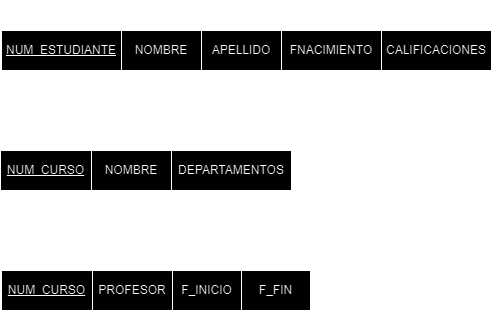
\includegraphics[scale = .5]{IMA/E1P1.png}    
    \end{center}
    \item[] Paso 2
    
    Se identifica que la entidad Sección es una entidad débil, ya que su existencia depende de la entidad Curso. Por lo tanto, se crea una nueva relación R para representar esta entidad débil.
    \begin{center}
        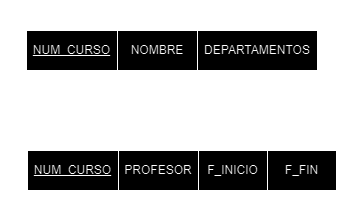
\includegraphics[scale = .5]{IMA/E1P2.png}    
    \end{center}
    
    \newpage
    \item[] Paso 3
    \thispagestyle{fancy} % Aplicar estilo de primera página  
    Por cada sección existe un único curso, por eso es uno a uno
    \begin{center}
        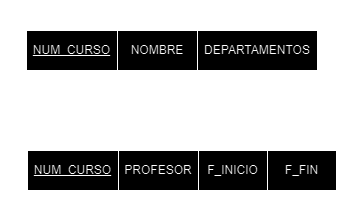
\includegraphics[scale = .5]{IMA/E1P2.png}    
    \end{center}
    
    \item[] Paso 4
    \thispagestyle{fancy} % Aplicar estilo de primera página  
    \begin{center}
        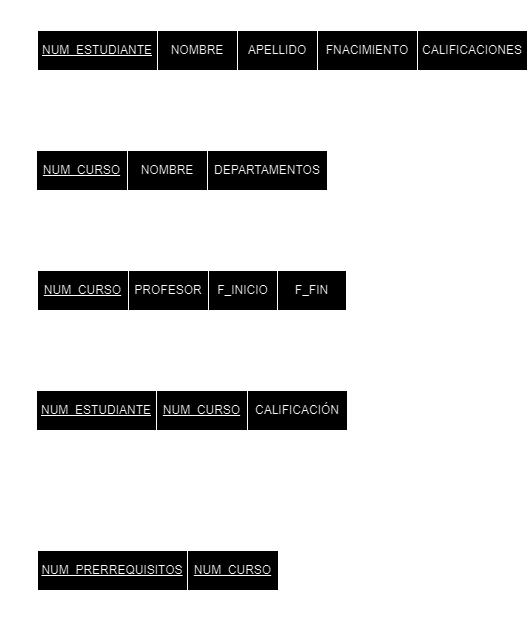
\includegraphics[scale = .5]{IMA/E1P4.png}    
    \end{center}
    
    \item[] Paso 5
    \thispagestyle{fancy} % Aplicar estilo de primera página  
    No hay relaciones binarias M:N en el esquema ER, por lo que este paso no se aplica.

    \newpage
    \item[] Paso 6

     El atributo calificaciones de la entidad Estudiante es multivaluado. Por lo tanto, se crea una nueva relación R para este atributo.
    \begin{center}
        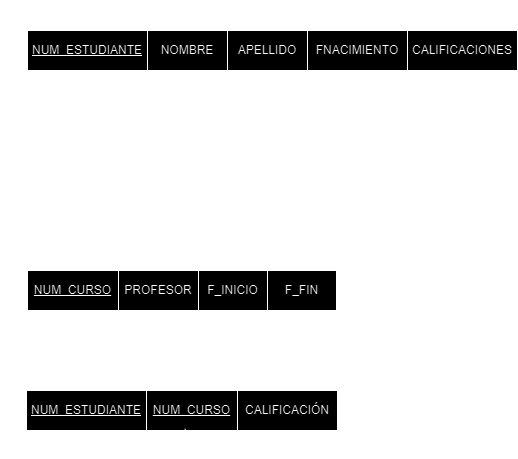
\includegraphics[scale = .4]{IMA/E1P6.png}    
    \end{center}
    
    \item[] Paso 7
    \thispagestyle{fancy} % Aplicar estilo de primera página  
    No hay tipos de asociaciones n-arias en el esquema ER
\end{enumerate}

\subsubsection*{Modelo entidad/asociación}
\begin{center}
    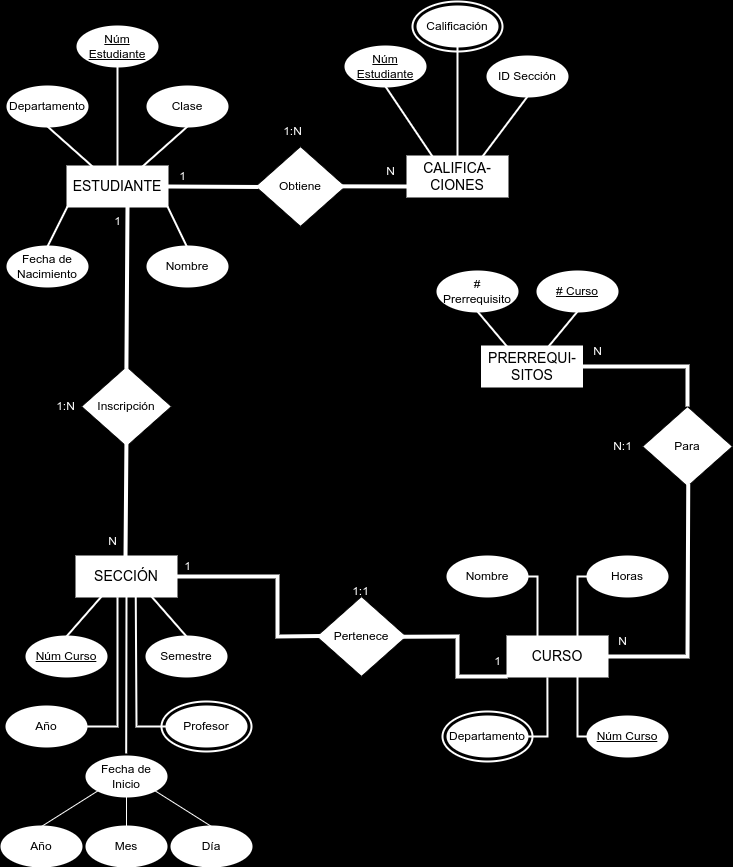
\includegraphics[scale = .5]{IMA/Ejercio1.png}    
\end{center}
\thispagestyle{fancy} % Aplicar estilo de primera página  
%%%%%%%%%%%%%%%%%%%%%%%%%%%%%%%%%%%%%%%%%%%%%%%%%%%%
%%%%%%%%%%%%%%%%%%%%%%%%%%%%%%%%%%%%%%%%%%%%%%%%%%%%
%%%%%%%%%%%%%%%%%%%%%%%%%%%%%%%%%%%%%%%%%%%%%%%%%%%%
\newpage
\section*{Ejercicio 2}
\textcolor{sun}{Empleando el algoritmo que se abordó en clase generar el modelo
relacional a partir del modelo entidad/asociación realizado en la práctica 3 (Consultorio). Mencionar y explicar con claridad cada paso realizado}
\thispagestyle{fancy} % Aplicar estilo de primera página

\subsubsection*{Modelo entidad/asociación}
\begin{center}
    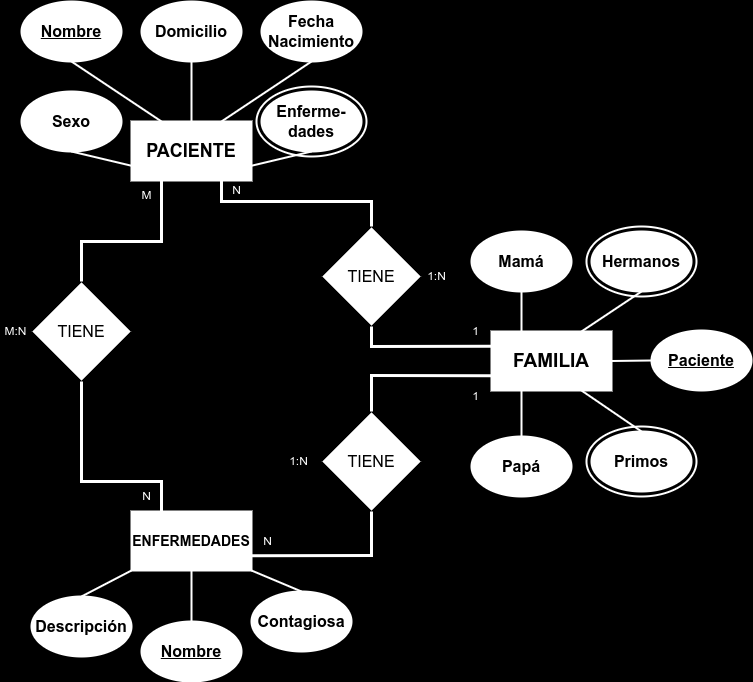
\includegraphics[scale = .5]{IMA/Ejercio2.png}
\end{center}

\subsubsection*{Modelo relacional}
\begin{enumerate}
  \item[] Paso 1
  \thispagestyle{fancy} % Aplicar estilo de primera página      
  Para cada tipo de entidad regular (fuerte) en el esquema ER, se crea una relación R que incluya todos los atributos simples de E.
  \begin{center}
    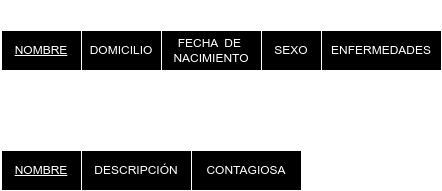
\includegraphics[scale = .5]{IMA/E2P1.png}
  \end{center}

  \item[] Paso 2
  \thispagestyle{fancy} % Aplicar estilo de primera página    
  Para cada tipo de entidad débil W en el esquema ER con un tipo de entidad propietaria E, 
  se crea una relación R y se incluyen todos los atributos simples 
  (o componentes simples de atributos compuestos) de W como atributos de R. En adición, 
  se incluye como atributos de llave foránea de R, a los atributos llave de la relación(es) 
  que corresponde al tipo de entidad(es) propietaria.
  \begin{center}
    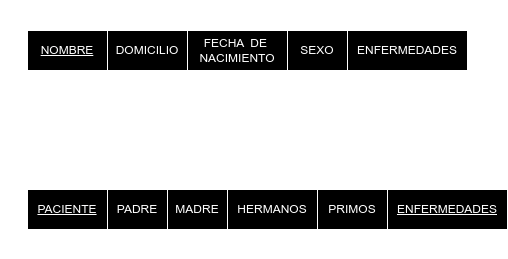
\includegraphics[scale = .5]{IMA/E2P2.png}
  \end{center}

  \item[] Paso 3
  \thispagestyle{fancy} % Aplicar estilo de primera página    
  No hay tipos de asociaciones binarias 1:1 en el esquema ER.

  \item[] Paso 4
  \begin{itemize}
    \item[] La relación 1:N entre Familia y Paciente se representa con una flecha que va de
            Familia a Paciente. Esta flecha indica que una familia solo puede tener un paciente,
            pero un paciente puede tener una o varias familias.
    \item[] La llave foránea de Familia a Enfermedades es enfermedades. Esta llave foránea se 
            utiliza para garantizar que cada familia solo pueda tener una lista de enfermedades.         

  \end{itemize}
  \begin{center}
    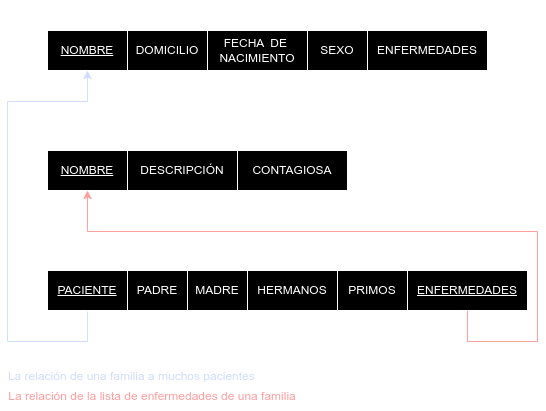
\includegraphics[scale = .5]{IMA/E2P4.png}
  \end{center}
  
  \item[] Paso 5
  \thispagestyle{fancy} % Aplicar estilo de primera página    
  \begin{center}
    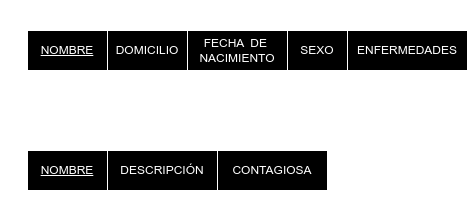
\includegraphics[scale = .5]{IMA/E2P5.png}
  \end{center}

  \item[] Paso 6
  
  \begin{center}
    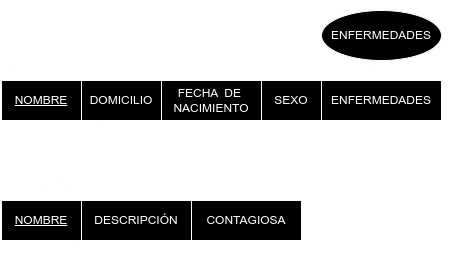
\includegraphics[scale = .5]{IMA/E2P6.png}
  \end{center}

  \item[] Paso 7
  \thispagestyle{fancy} % Aplicar estilo de primera página    
  No hay tipos de asociaciones n-arias en el esquema ER.

\end{enumerate}


\thispagestyle{fancy} % Aplicar estilo de primera página    
\section*{Cuestionario}
\begin{enumerate}
    \item \textcolor{sun}{¿Cuáles son las principales características de los modelos relacionales?} 

    
    Los modelos relacionales son una forma de representar datos y su estructura en una base de datos. Sus principales características son:
    \begin{itemize}
        \item Utilizan tablas (relaciones) para organizar los datos.
        \item Cada fila en una tabla representa una entidad única.
        \item Las columnas en la tabla representan atributos o características de la entidad.
        \item Establecen relaciones entre tablas utilizando claves primarias y claves foráneas.        
        \item Soportan consultas SQL para recuperar y manipular datos.
    \end{itemize}

    \item \textcolor{sun}{¿Cuál es la principal diferencia entre el modelo entidad relación y el modelo relacional? } 
     
    La principal diferencia entre el modelo entidad-relación y el modelo relacional radica en su nivel de abstracción y enfoque:
    \begin{itemize}
        \item El modelo entidad-relación se enfoca en la representación de entidades, atributos y relaciones entre ellas de una manera más conceptual y visual, utilizando diagramas ER.
        \item El modelo relacional se centra en la representación de datos de manera tabular, utilizando tablas con filas y columnas para organizar la información. Se basa en la teoría de conjuntos y álgebra relacional.
    \end{itemize}

    \item \textcolor{sun}{¿Para qué sirven los modelos relacionales?} 

    
    Los modelos relacionales sirven para gestionar y organizar datos de manera estructurada en una base de datos. Sus usos principales incluyen:
    \begin{itemize}
        \item Almacenar y gestionar información en aplicaciones empresariales.
        \item Facilitar consultas y análisis de datos utilizando lenguaje SQL.
        \item Mantener la integridad de los datos a través de restricciones y relaciones.
        \item Permitir la recuperación eficiente de datos.
        \item Apoyar la escalabilidad y la seguridad de los sistemas de bases de datos.
    \end{itemize}
    \thispagestyle{fancy} % Aplicar estilo de primera página    
\end{enumerate}


%\newpage
%\thispagestyle{fancy} % Aplicar estilo de primera página
%\thispagestyle{firstpage} % Aplicar estilo de primera página
%\printbibliography[title={Bibliografia:}]%


%\printbibliography


%\newpage
%\thispagestyle{fancy} % Aplicar estilo de primera página
%\NoBgThispage % Quita el fondo de la pagina

%-----------------------------------------------------------------|
\end{document}%----------------------FIN DEL DOCUMENTO------------| 